%%%%%%%%%%%%%%%%%%%%%%%%%%%%%%%%%%%%%%%%%%%%%%%%%%%%%%%%%%%%%%%%%%%%%%%%%%%%
% AGUJournalTemplate.tex: this template file is for articles formatted with LaTeX
%
% This file includes commands and instructions
% given in the order necessary to produce a final output that will
% satisfy AGU requirements, including customized APA reference formatting.
%
% You may copy this file and give it your
% article name, and enter your text.
%
%
% Step 1: Set the \documentclass
%
% There are two options for article format:
%
% PLEASE USE THE DRAFT OPTION TO SUBMIT YOUR PAPERS.
% The draft option produces double spaced output.
%

%% To submit your paper:
\documentclass[draft]{agujournal2019}
\usepackage{url} %this package should fix any errors with URLs in refs.
\usepackage{lineno}
\usepackage{color}
\graphicspath{ {figures/} }
\linenumbers
%%%%%%%
% As of 2018 we recommend use of the TrackChanges package to mark revisions.
% The trackchanges package adds five new LaTeX commands:
%
%  \note[editor]{The note}
%  \annote[editor]{Text to annotate}{The note}
%  \add[editor]{Text to add}
%  \remove[editor]{Text to remove}
%  \change[editor]{Text to remove}{Text to add}
%
% complete documentation is here: http://trackchanges.sourceforge.net/
%%%%%%%

\draftfalse

%% Enter journal name below.
%% Choose from this list of Journals:
%
% JGR: Atmospheres
% JGR: Biogeosciences
% JGR: Earth Surface
% JGR: Oceans
% JGR: Planets
% JGR: Solid Earth
% JGR: Space Physics
% Global Biogeochemical Cycles
% Geophysical Research Letters
% Paleoceanography and Paleoclimatology
% Radio Science
% Reviews of Geophysics
% Tectonics
% Space Weather
% Water Resources Research
% Geochemistry, Geophysics, Geosystems
% Journal of Advances in Modeling Earth Systems (JAMES)
% Earth's Future
% Earth and Space Science
% Geohealth
%
% ie, \journalname{Water Resources Research}

\journalname{JGR: Space Physics}


\begin{document}

\title{Microburst Scale Size Distribution Derived with AeroCube-6}

%% ------------------------------------------------------------------------ %%
%
%  AUTHORS AND AFFILIATIONS
%
%% ------------------------------------------------------------------------ %%

\authors{M. Shumko\affil{1}, T.P. O'Brien\affil{2}, J. Sample\affil{1}, A. Johnson\affil{1}, D.L. Turner\affil{2}, J.B. Blake\affil{2}, B.A. Griffith\affil{1}, S. Claudepierre\affil{2}, O. Agapitov\affil{3}}


\affiliation{1}{Department of Physics, Montana State University, Bozeman, Montana, USA}
\affiliation{2}{Space Science Applications Laboratory, The Aerospace Corportation, El Segundo, California, USA}
\affiliation{3}{Space Sciences Laboratory, University of California berkeley, Berkeley, California, USA}

\correspondingauthor{M. Shumko}{msshumko@gmail.com}

%% Keypoints, final entry on title page.
%  List up to three key points (at least one is required)
%  Key Points summarize the main points and conclusions of the article
%  Each must be 100 characters or less with no special characters or punctuation and must be complete sentences

\begin{keypoints}
\item Microburst scale size in low Earth orbit and the magnetic equator was estimated.
\item Majority of microbursts in low Earth orbit have a scale size on the order of 10 km.
\item The majority of microbursts correspond to the correlation scale of \textcolor{red}{high amplitude?} whistler-mode chorus waves at the magnetic equator.
\end{keypoints}

%% ------------------------------------------------------------------------ %%
%
%  ABSTRACT
%
% A good abstract will begin with a short description of the problem
% being addressed, briefly describe the new data or analyses, then
% briefly states the main conclusion(s) and how they are supported and
% uncertainties.
%% ------------------------------------------------------------------------ %%

%% \begin{abstract} starts the second page

\begin{abstract}
Microbursts are an impulsive increase of electrons from the radiation belts into the atmosphere and has been directly observed in low Earth orbit and upper atmosphere. Microburst are believed to be generated by wave-particle scattering between whistler mode waves and radiation belt electrons. Prior work has estimated that microbursts are capable of rapidly depleting the radiation belt electrons on the order of a day, hence their role to radiation belt electron losses must be considered. Radiation belt electron losses due to microbursts is not well understood, and more work is necessary to accurately quantify their contribution. To further address this question we present a statistical study of microburst scale sizes using the pair of AeroCube-6 CubeSats. The microburst scale size distribution in low Earth orbit and the magnetic equator was derived. In low Earth orbit, \textcolor{red}{the majority of microbursts were found to have a size of less than a few tens of km with a minority of microbursts observed at a separation above 50 km. When mapped to the magnetic equator, the microburst scale size distribution corresponded to the high amplitude whistler mode chorus scale size derived in prior literature.}
\end{abstract}

\section{Plain Language Summary}
https://sharingscience.agu.org/creating-plain-language-summary/



%% ------------------------------------------------------------------------ %%
%
%  TEXT
%
%% ------------------------------------------------------------------------ %%

%%% Suggested section heads:
% \section{Introduction}
%
% The main text should start with an introduction. Except for short
% manuscripts (such as comments and replies), the text should be divided
% into sections, each with its own heading.

% Headings should be sentence fragments and do not begin with a
% lowercase letter or number. Examples of good headings are:

% \section{Materials and Methods}
% Here is text on Materials and Methods.
%
% \subsection{A descriptive heading about methods}
% More about Methods.
%
% \section{Data} (Or section title might be a descriptive heading about data)
%
% \section{Results} (Or section title might be a descriptive heading about the
% results)
%
% \section{Conclusions}


\section{Introduction}
Since the discovery of the Van Allen radiation belts in the 1960s by \citeA{Allen1959} and \citeA{Vernov1960}, decades of research has made headway in understanding the dynamics of particle acceleration and loss mechanisms. One of these mechanisms is wave-particle scattering between whistler-mode chorus waves and electrons which has been modeled and observed as a source of electron acceleration and loss \cite{Abel1998_1, Meredith2002, Horne2003, Thorne2005, Millan2007, Bortnik2008}. Whistler-mode chorus waves are typically generated by a temperature anisotropy of low energy electrons up to tens of kiloelectronvolts (keV) \cite{Li2009b}. \citeA{Li2009} found that chorus waves predominately occur in $\sim 6-12$ magnetic local times (MLT).

Whistler mode chorus is widely believed to cause electron precipitation termed microbursts \cite{Millan2007}. Microbursts are a subsecond impulse of electrons that are observed by high altitude balloons and satellites in low Earth orbit (LEO) on the radiation belt magnetic footprints, $\sim 4 - 8$ L-shell (L) \cite{Anderson1964, Parks1967, Woodger2015, Lorentzen2001a, Lorentzen2001b, O'Brien2003, O'Brien2004, Lee2005, Lee2012, Crew2016, Breneman2017, Mozer2018}. Microburst’s role as a radiation belt electron loss mechanism has been estimated to be significant, with total radiation belt electron depletion due to microbursts estimated to be on the order of a day \cite{Lorentzen2001b, O'Brien2004, Thorne2005, Breneman2017}. 

One of the unknown characteristics of microbursts that is critical to better quantify the role of microbursts as a loss mechanism is their size. \textcolor{red}{Move "why we should care?" to end of paragraph?} Microburst size, together with their occurrence frequency \textcolor{red}{anything else?} are necessary parameters to more accurately quantify their contribution to radiation belt electron losses. Furthermore, by comparing the microburst scale size distribution mapped to the magnetic equator to the wave scale sizes estimated in prior litera	ture, the dominant scattering mechanism can be identified. Historically there have been various case studies that estimated microburst scale size. \citeA{Parks1967} found that the scale size of mostly low energy microbursts to be $40 \pm 14$ km. \citeA{Blake1996} found a microburst with a size of a few tens of km using the the Solar Anomalous and Magnetospheric Particle Explorer (SAMPEX) and concluded that typically microbursts are less than a few tens of electron gyroradii in size (order of a few km). \citeA{Dietrich2010} also used SAMPEX in another case study and concluded that the observed microbursts were smaller than $4$ km. More recently, \citeA{Crew2016} used the Focused Investigation of Relativistic Electron Bursts: Intensity, Range, and Dynamics CubeSats and found an example of a microburst larger than 11 km, and \citeA{Shumko2018a} found a microburst with a size greater than $ 51 \pm 1$ km. The large variance in prior results imply that there is a distribution of microburst scale sizes that this study aims to estimate.

This study estimates the microburst scale size distributions in LEO and the magnetic equator and compares it to the scale size of the progenitor waves. The twin AeroCube-6 (AC6) CubeSats which took data together for three years with varying spacecraft separation between 2 and 800 km are utilized for this study. We first introduce the AC-6 mission including their orbit and instrumentation. Then we describe the procedure undertaken to identify microbursts observed by each spacecraft and how they are combined to make a list of the temporally coincident microbursts. Next, the procedure used to estimate the microburst scale size distributions in LEO and the magnetic equator is explained. Lastly, we summarize and compare these results to the microburst scale sizes estimated in prior literature and infer the properties of the whistler-mode chorus waves that are believed to cause microbursts. 

\section{Instrumentation}
The AC6 mission consists of a pair of 0.5U (10x10x5 cm) CubeSats built by the Aerospace Corporation and launched on June 19th, 2014 into a 620 x 700 km, 98 degree inclination orbit. The two satellites, designated as AC6-A and AC6-B separated after launch and drifted apart. AC6 has an active attitude control system which allows them to change their differential drag to allow fine separation control. Figure 1a shows the AC6 separation for the duration of the mission.

Each AC6 unit is equipped with a three Aerospace microdosimeters (licensed to Teledyne Microelectronics, Inc). The dosimeter used for this study is dos1 and is identical on both AC6 units. Dos1 has a 30 keV electron threshold and samples at 10 Hz. The AC6 orbit is in the dawn-dusk magnetic local times (MLTs) and Fig. 1b shows the number of good 10 Hz samples taken simultaneously by AC6 as a function and L and MLT. Good samples are samples which have a 0 data quality flag. More detailed technical information regarding the AC6 mission can be found in \citeA{Obrien2016}.

\begin{figure}
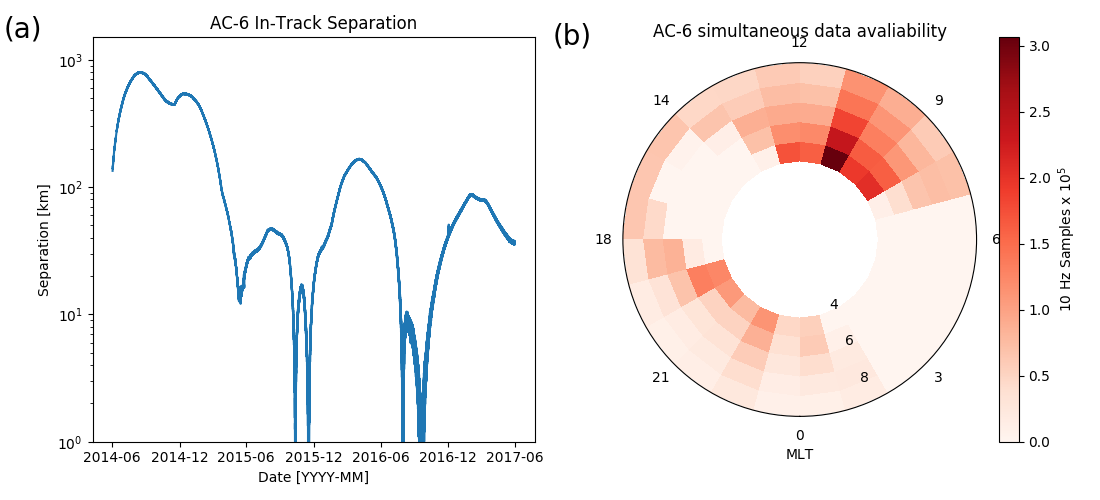
\includegraphics[width=\textwidth]{fig1.png}
\caption{AC6 mission distributions for (a) spacecraft separation and (b) number of simltaneous 10 Hz samples as a function of L and MLT.} \label{fig1}
\end{figure}

\section{Methodology}
\subsection{Microburst Detection}
The first step to find microbursts observed simultaneously by both spacecraft is to identify them from each spacecraft separately. We have detected microbursts with two different methods that yielded quantitatively similar results. The first method is the burst parameter \cite{O'Brien2003}. This algorithm has been successfully used in other microburst studies, mainly with the microbursts observed by the Solar Anomalous and Magnetospheric Particle Explorer add citations. For AC6, we found that a burst parameter threshold of 5 has good tradeoff between false positive and false negative microburst detections. \textcolor{red}{Talk about the wavelet based detector as well?}

The transmitters on AC6 can cause unphysical count impulses in the dosimeters that resembles periodic trains of microbursts. These false detections were removed to remove their bias. One source of transmitter noise was observed at times when AC6 was in contact with the ground stations above mainland US for data downloads and commanding thus the mostly low L detections made above the US were discarded. 

Another source of noise is crosslink transmissions between the AC6 units. These transmissions occurred when either spacecraft transitioned from the survey mode to 10 Hz mode. This noise is sometimes not caught by the data quality flag, so the following empirically-derived criteria was developed to remove those detections. The dosimeter with a 250 keV nominal electron threshold, dos2 was used because it had a similar response to noise while rarely responded to microbursts. Since the transmitter noise is very periodic, cross-correlation (CC) and autocorrelation (AC) methods were applied to the dos1 and dos2 time series. Detections were removed if the following two criteria were met: either dos1 or dos2 time series had a AC peak at a 0.2 or 0.4 s lag, and the dos1-dos2 CC was greater than 0.9. The AC lag criteria alone sometimes falsely removed legitimate trains of microbursts, so the second criteria insured that the detection was removed if there was a very high correlation across an order of magnitude in energy.

The lists of microbursts observed by either AC6 unit were merged into a temporally coincident list with the following procedure. \textcolor{red}{Show the microburst detection cartoon I`ve showed in conferences?} The general idea is that a microburst detection on one spacecraft will CC well will the time series from the other spacecraft if it observed a similar microburst, and poorly if there was no microburst observed by the other spacecraft. Each microburst detection made by either spacecraft was CC with the time series from the other spacecraft. Windows of 1 and 1.2 s were used to CC the time series. Different window sizes were used to account for numerical uncertainty due to Poisson noise. Microbursts detections with a CC above 0.8 were considered temporally coincident. This CC threshold was chosen as it is low enough to identify temporally coincident microbursts superposed with noise, and high enough to reject most non-coincident events. Figure \ref{fig2}, panels (a), (c), and (e) show examples of microbursts observed by both AC6 units when they were separated by 6, 17, and 69 km, respectively. 

The last CC criteria required that the temporal CC must be greater than the spatial CC + 0.3. The spatial CC was calculated by shifting the AC6-B time series by the in-track lag to CC in latitude. This criteria was applied to remove curtains, spatially stationary and narrow in latitude structures obsered by AC6 \cite{Blake2016} and sometimes appear as microbursts. Figure \ref{fig2}, panels (b), (d), and (f) show the AC6 spatially aligned time series to confirm that the three cases shown were indeed microbursts. The coincident microburst list was then spot checked by two authors to any remove poorly correlated events. Considering the CC criteria and data availability, 662 confirmed simultaneous microburst detections are used to calculate the microburst scale size distribution in the following section.

\begin{figure}
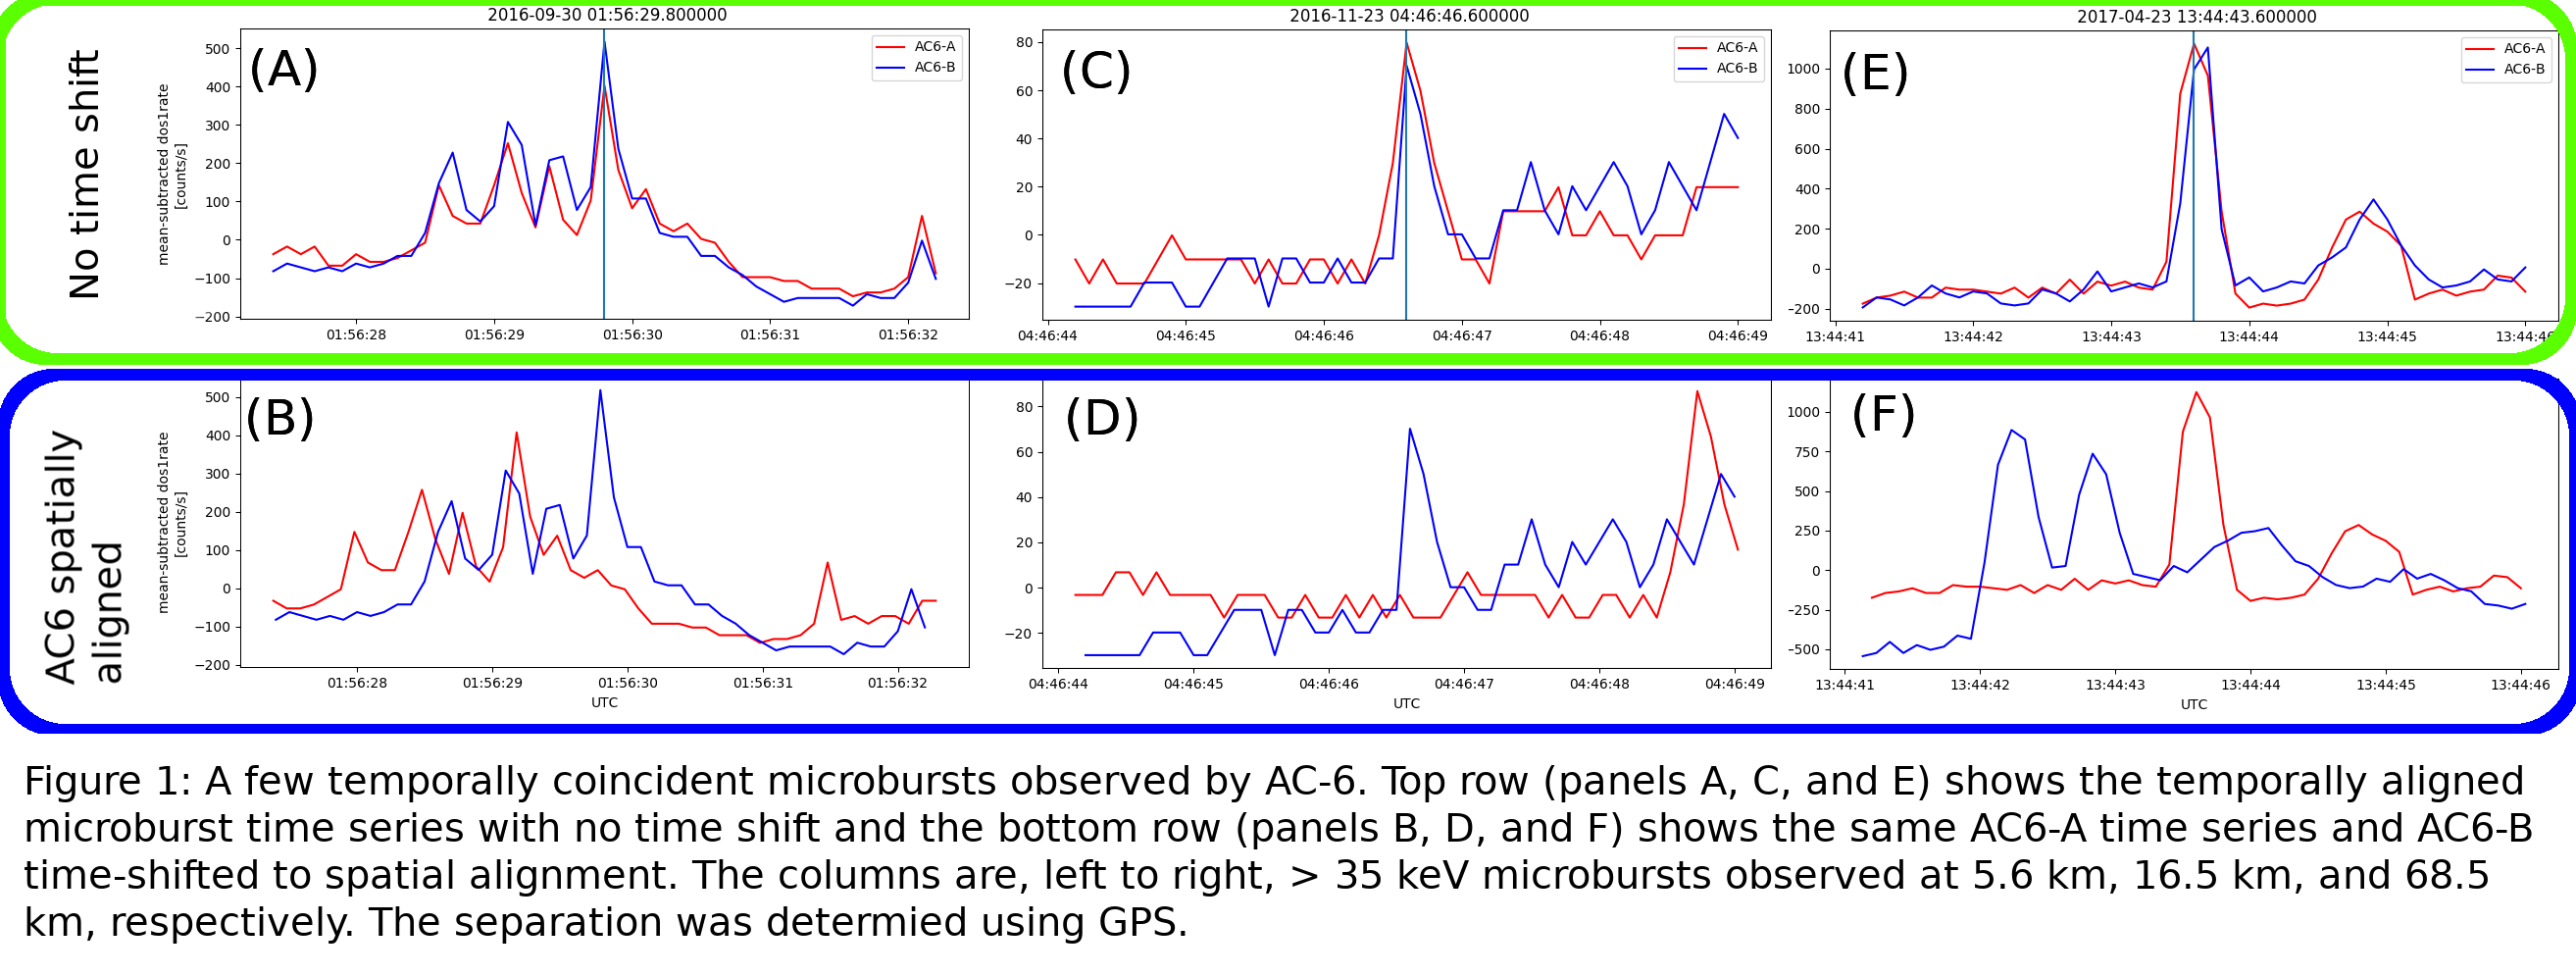
\includegraphics[width=\textwidth]{fig2.png}
\caption{Examples of microbursts observed simulatenously by AC6. Panels (a), (c) and (e) shows the temporally-aligned time series at spacecraft separations of 5.6 km, 16.5 km, and 68.5 km, respectively. Pabels (b), (d), and (f) show the spatially aligned time series corresponding to the time series in the same column. The clear temporal correlation and lack of spatial correlation demonstrates that these events are microbursts.} 
\label{fig2}
\end{figure}
	

\subsection{Microburst Size Distribution in LEO and Magnetic Equator}\label{microburst_distribution}
When AC6 observes a coincident microburst at a separation $d$, the microburst`s size must be greater than $d$. This idea is similar to \citeA{Joy2002} who investigated the most probable Jovian bow shock and magnetopause standoff distances. Following the arguments presented in Section 4 in \citeA{Joy2002}, we investigate the dependence of the number of coincident microbursts observed above $d$, as a function of $d$ that is the microburst complementary cumulative distribution $F(d)$.  If P(A) is the probability that a microburst is larger than $d$ and P(B) is the probability that AC6 is separated by $d$, then the fraction of microbursts observed at $d$ is the conditional probability $P(A \ \vert \ B)$. Using Bayes’ theorem, 
\begin{equation}
P(A \ \vert \ B) = \frac{P(A \ \& \ B)}{P(B)}
\end{equation} where $P(A \ \& \ B)$ is the joint probability. Since the AC6 separation is independent of microburst size, $P(A \ \& \ B) = P(A)P(B)$. Hence

\begin{equation}
P(A \ \vert \ B) = \frac{P(A)P(B)}{P(B)} = P(A)
\end{equation} and \textcolor{red}{seems like a big jump in logic...}

\begin{equation}
F(d) = \frac{N(d)}{N(0)}
\end{equation} where $N(d)$ is the number of microbursts observed by AC6 above separation $d$ and is defined as

\begin{equation}
N(d) = \sum_{\mathrm{bins > d}} n_{bin} \frac{S_{max}}{S_{bin}}
\end{equation} where $n_{bin}$ is the number of microbursts detected by both AC6 units in that bin. The normalization term $S_{max}/S_{bin}$ is a ratio of the number of samples observed in the most sampled bin to the number of samples in the current bin. This normalization factor corrects for AC6's non-uniform sampling in separation. With this normalization, $F(d)$ can be interpreted as the fraction of microbursts observed above $d$ assuming AC6 sampled evenly in separation. Microburst $F(d)$ in LEO is shown by the black curve in Fig. \ref{fig3}a for the entire radiation belt ($4 < \mathrm{L}< 8$) and split into one L-wide bins with the colored curves. The separation bin width in Fig. \ref{fig3} is 5 km. To check for bias in $F(d)$ due to the separation bins, other bin widths and offsets were used to calculate $F(d)$. Bin widths as large as the size of the features in $F(d)$ ($20-30$ km) and bin offsets smaller than the bin width did not effect the curves in Fig. \ref{fig3}a.

The overall trend in Fig. \ref{fig3}a consists of a sudden cumulative probability drop off, followed by a shoulder up to about 70 km where the cumulative distribution drops to nearly zero. The shaded region around the black curve shows the standard error due to counting statistics. The uncertainty due to false coincidence events i.e. two unrelated microbursts randomly lining up in time was also considered. For each coincident microburst the microburst duty cycle in a one minute window ($\approx 1 L$) was calculated. The false coincidence probability is then the square of the duty cycle and was found to be less than 5\% for the majority of these events. The false coincidence probability for each microburst was then used to randomly remove microbursts and $F(d)$ was recalculated in $1000$ trials. The uncertainty in $F(d)$ with microbursts randomly removed was much smaller than the uncertainty due to counting statistics alone. Lastly, Fig. \ref{fig3}b shows the microburst probability density derived numerically from $F(d)$ and shows a peak at spacecraft separations of $d < 20 $ km as well as a peak between 70-80 km. 

To estimate the equatorial microburst scale size distribution, the microburst events were mapped to the magnetic equator using the Olson-Pfitzer magnetic field model \cite{Olson1982} which is implemneted with a Python wrapper for IRBEM-Lib \cite{irbem}. Once all microburst events and spacecraft separations were mapped to the magnetic equator, the procedure to estimate $F(d)$ is identical to the LEO scale size distribution with the normalization being the only distinction. The normalization factors were calculated by mapping every AC6 time series sample taken simultaneously to the magnetic equator and binning them by separation into 100 km wide bins. Figure \ref{fig4} shows the equatorial microburst scale size distribution in the same format as Fig. \ref{fig3}. Similar to the microburst probability density in LEO, most of the microburst probability density was observed when the AC6 equatorial separation was less than 300 km. 

The results in Figs. \ref{fig3} and \ref{fig4} show the fraction of microbursts observed above a spacecraft separation. These measurements do not fully represent the microbursts size distribution due to the compounding effects from the range of microburst sizes and the random locations of microbursts with respect to AC6. Thus modeling is necessary to capture the influence of these statistical effects on two-point measurements.

\begin{figure}
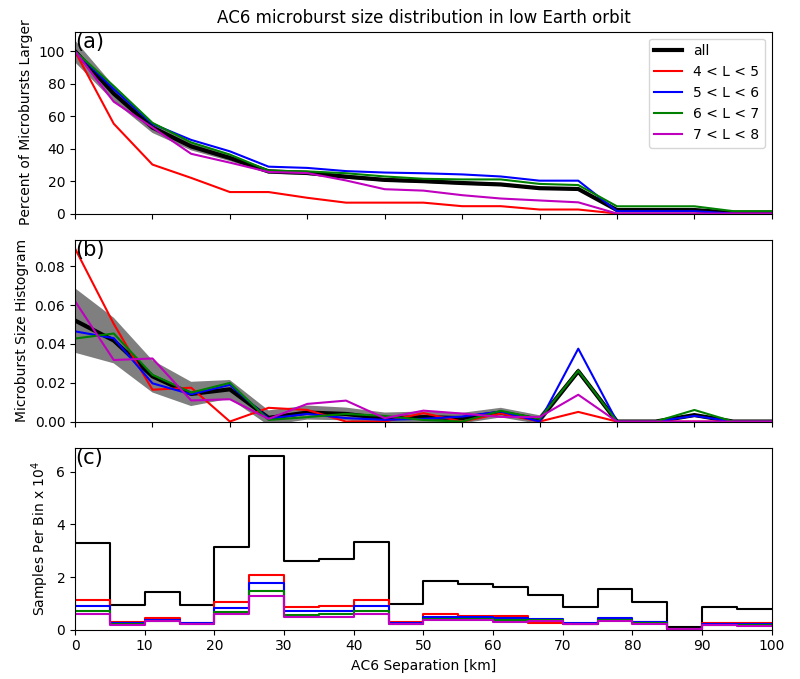
\includegraphics[width=\textwidth]{fig3.png}
\caption{Fraction of microbursts greater than the spacecraft separation as a function of separation in LEO. Panel (a) shows the fraction of microbursts observed above that separation. Panel (b) shows the microburst probability density as a function of separation. Lastly, panel (c) shows the number of simultaneous samples AC6 observed as a function of separation. The colored lines show the distributions binned by L, and the thick black curve shows the fraction of microbursts observed above a separation in the entire radiation belt ($4 < L < 8$). The gray shading around the black curve shows the uncertainty due to counting statistics.}
\label{fig3}
\end{figure}

\begin{figure}
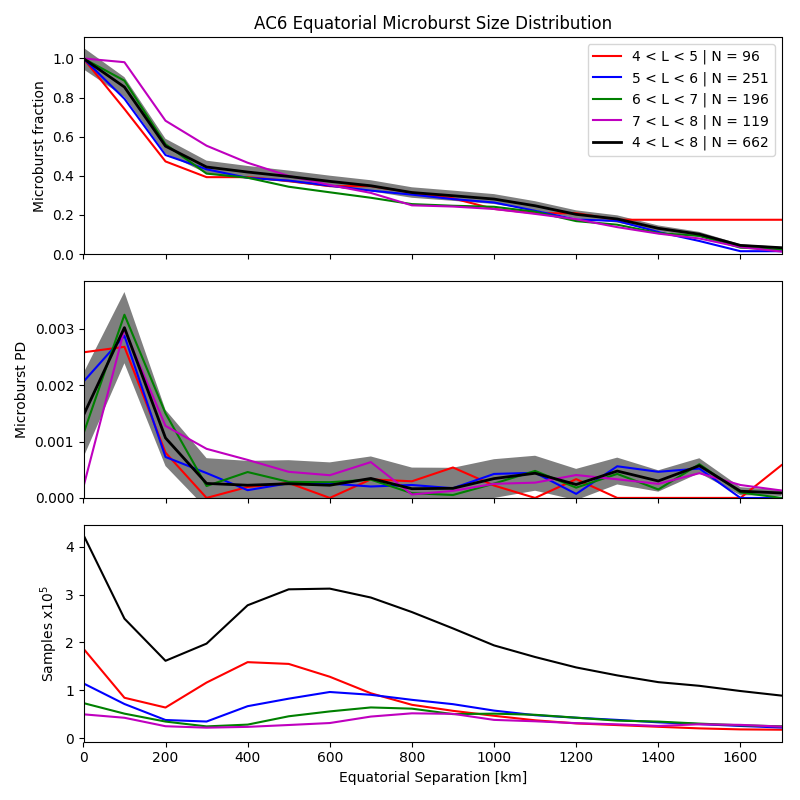
\includegraphics[width=\textwidth]{fig4.png}
\caption{Microburst scale size distribution in the same format as Fig. \ref{fig3} and mapped to the magnetic equator.} 
\label{fig4}
\end{figure}

\section{Modeling the Microburst Size Distribution}
\textcolor{blue}{
TO-DO
\begin{itemize}
\item Talk about the brute force MC model.
\item Show a LEO CDF model assuming a fixed-sized microburst population.
\item Decide if I should show a two-fixed-sized microburst population or a microburst CDF.
\item Show the residuals in the plots.
\end{itemize}
}

An analytic and Monte Carlo (MC) models were developed to account for the statistical effects of random microburst sizes and locations in the vicinity of AC6. \textcolor{red}{FINISH THIS!}

 In this section we discuss the model developed to understand the relation between $F(d)$ shown in Fig. \ref{fig3}a and the true distribution of microburst sizes. This relation is not immediately clear since microbursts are randomly scattered around the spacecraft location during a radiation belt pass, and have an unknown geometry. We address these issues with a Monte Carlo (MC) and analytic models and we assume that microbursts are circular with a radius $r$. For simplicity we first assume that all microbursts are the same $r$ and then generalize their size to a microburst probability density function (PDF). 

The MC model first randomly scattered $10^5$ microburst centers in a 400 x 400 km grid around the spacecraft. Spacecraft A is placed at the origin, and spacecraft B is placed along the positive y-axis at the same distances from the origin as the separation bins, $D$ used in Section \ref{microburst_distribution}. Then the number of simultaneously observed microbursts at each spacecraft B distance in $D$ was counted. The modeled fraction of microbursts is then
\begin{equation}
F(d) = \frac{\sum_{d > D} n_{d} }{\sum_{d \in D} n_{d}}.
\end{equation} and an example run of the MC model with a 40 km diameter microburst population is shown in Fig. \ref{fig5}b.

The analytic model, while identical to the MC model, highlights the concepts connecting the microburst size distribution and $F(d)$. The fundamental idea is that given a spacecraft separation $d$ and microburst radius $r$, there exists an area $A$ with the property that for any microburst center inside it will be observed by both spacecraft. The geometry of this model and $A$ is shown in Fig. \ref{fig5}a. Figure \ref{fig5}a shows the two spacecraft as blue cubes and two identical microbursts of radius $r$ shown by the black circles. This extreme case shows that the microburst centers are $r$ from either spacecraft, the maximum distance away from the spacecraft and be observed by both units. Microbursts with centers closer to the spacecraft will also be observed by both spacecraft. 

Now we use the original geometry and rotate the right circle clockwise about the top spacecraft until the bottom spacecraft is outside the rotated circle. The circle's origin will trace a curve that connects the two black circle centers which is shown by the lower red-dotted line. This problem is symmetric and we can also rotate the right circle counter-clockwise about the lower spacecraft in the same manner and the center will trace out the upper red-dotted curve. The two red-dotted lines outline $A$ and if a microburst center lies anywhere in $A$, it will be observed by both spacecraft. 

How do we find $A$? It must be a function of $r$ and $d$ and we need to find $A(r, d)$. Instead of tracing out the red-dotted curves between the black circles' centers, the black circles are rotated through a full revolution. This will trace out the circles comprised of the red and red-dotted curves. These centers of the two circles are separated by $d$ and the radius of the circles is $r$ and $A$ is the area where the two circles intersect and is given by 

\begin{equation}
A(r, d) = 2r^2 \cos^{-1}{\Big( \frac{d}{2r} \Big)} - \frac{d}{2} \sqrt{4r^2 - d^2}.
\end{equation} \textcolor{red}{Cite anything? Wolfram: http://mathworld.wolfram.com/Circle-CircleIntersection.html} Lastly, the fraction of microbursts as a function of separation is given by 
\begin{equation}
F(r, d) = \frac{\sum_{d > D} A(r, d)}{\sum_{d \in D} A(r, d)}.
\end{equation} Where the denominator is the normalization factor. An example of the analytic $F(r=20 \ \mathrm{km}, d)$ is shown in Fig. \ref{fig5}b with the dashed blue curve. 

%Lastly we calculate the microburst CDF. Compare the number of microbursts of size $r$ that %would be observed by both spacecraft at a spacecraft separation $d_0$ and $d_1$ with $d_0 < d_1$. The fraction of the number of microbursts observed at $d_1$ compared to $d_0$ is just the fraction of the areas since microbursts are uniformly distributed around the two spacecraft. Now we can compare these areas to the CDF derived from the data. For now assume a fixed microburst scale size, and a range of separations $D$. Then 


\begin{figure}
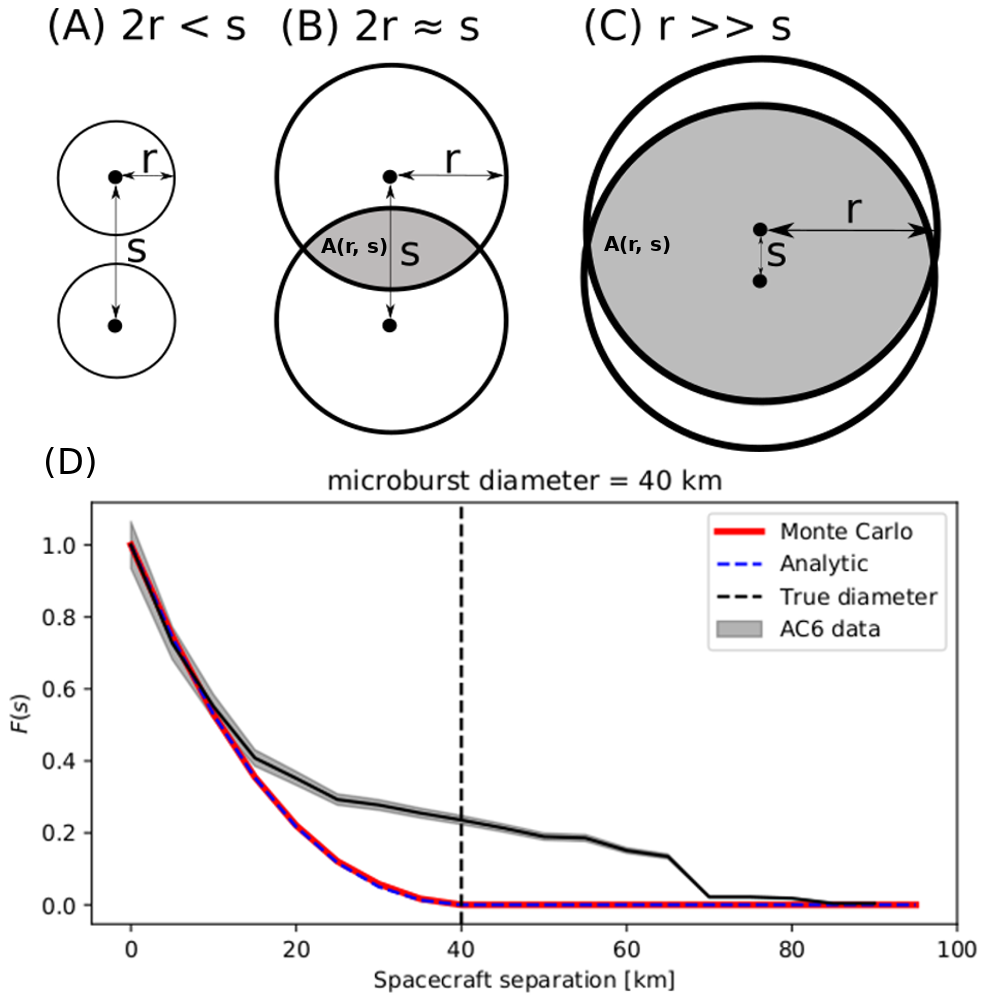
\includegraphics[width=\textwidth]{fig5.png}
\caption{Modeling a single-sized microburst distribution. Panel A shows the geometry of the analytic model. Assuming a microburst radius $r$ (microbursts shown with black circles) and spacecraft separation $d$, the area $A$ shows all possible microburst center locations where a microburst will be simultaneously observed by both spacecraft. The two black circles show the most distant microburst location that is observed by both spacecraft. The red solid and dashed curves are found by rotating either of the black circles about the top and bottom spacecraft. Panel B shows the microburst fraction, $F(d)$ as a function of separation from the AC6 data in solid black. The red and dashed blue curves show the $F(d)$ assuming all microbursts have a 40 km diameter.} 
\label{fig5}
\end{figure}


\section{Discussion}
\textcolor{blue}{
TO-DO
\begin{itemize}
\item Discuss the significance of the peaks in the LEO CDF \& PDF.
\item Discuss the secondary peak.
\item Talk about how these sizes fit in with prior work and how they can be used to estimate microburst loss rates.
\item Maybe add a plot with Oleksiy's data?
\item Use the wave data to interpret the equatorial scale size distribution. Is the < 200 km peak due to high amplitude waves, or is it just that waves are most common at those scales?
\end{itemize}
}

\section{Conclusions}

%%

%  Numbered lines in equations:
%  To add line numbers to lines in equations,
%  \begin{linenomath*}
%  \begin{equation}
%  \end{equation}
%  \end{linenomath*}



%% Enter Figures and Tables near as possible to where they are first mentioned:
%
% DO NOT USE \psfrag or \subfigure commands.
%
% Figure captions go below the figure.
% Table titles go above tables;  other caption information
%  should be placed in last line of the table, using
% \multicolumn2l{$^a$ This is a table note.}
%
%----------------
% EXAMPLE FIGURE
%
%
% Giving latex a width will help it to scale the figure properly. A simple trick is to use \textwidth. Try this if large figures run off the side of the page.
% \begin{figure}
% \noindent\includegraphics[width=\textwidth]{anothersample.png}
%\caption{caption}
%\label{pngfiguresample}
%\end{figure}
%
%
%
% If you get an error about an unknown bounding box, try specifying the width and height of the figure with the natwidth and natheight options.
% \begin{figure}
% \noindent\includegraphics[natwidth=800px,natheight=600px]{samplefigure.pdf}
%\caption{caption}
%\label{pdffiguresample}
%\end{figure}
%
%
% PDFLatex does not seem to be able to process EPS figures. You may want to try the epstopdf package.
%
%
%
% ---------------
% EXAMPLE TABLE
%
% \begin{table}
% \caption{Time of the Transition Between Phase 1 and Phase 2$^{a}$}
% \centering
% \begin{tabular}{l c}
% \hline
%  Run  & Time (min)  \\
% \hline
%   $l1$  & 260   \\
%   $l2$  & 300   \\
%   $l3$  & 340   \\
%   $h1$  & 270   \\
%   $h2$  & 250   \\
%   $h3$  & 380   \\
%   $r1$  & 370   \\
%   $r2$  & 390   \\
% \hline
% \multicolumn{2}{l}{$^{a}$Footnote text here.}
% \end{tabular}
% \end{table}

%% SIDEWAYS FIGURE and TABLE
% AGU prefers the use of {sidewaystable} over {landscapetable} as it causes fewer problems.
%
% \begin{sidewaysfigure}
% \includegraphics[width=20pc]{figsamp}
% \caption{caption here}
% \label{newfig}
% \end{sidewaysfigure}
%
%  \begin{sidewaystable}
%  \caption{Caption here}
% \label{tab:signif_gap_clos}
%  \begin{tabular}{ccc}
% one&two&three\\
% four&five&six
%  \end{tabular}
%  \end{sidewaystable}

%% If using numbered lines, please surround equations with \begin{linenomath*}...\end{linenomath*}
%\begin{linenomath*}
%\begin{equation}
%y|{f} \sim g(m, \sigma),
%\end{equation}
%\end{linenomath*}

%%% End of body of article

%%%%%%%%%%%%%%%%%%%%%%%%%%%%%%%%
%% Optional Appendix goes here
%
% The \appendix command resets counters and redefines section heads
%
% After typing \appendix
%
%\section{Here Is Appendix Title}
% will show
% A: Here Is Appendix Title
%
%\appendix
%\section{Here is a sample appendix}

%%%%%%%%%%%%%%%%%%%%%%%%%%%%%%%%%%%%%%%%%%%%%%%%%%%%%%%%%%%%%%%%
%
% Optional Glossary, Notation or Acronym section goes here:
%
%%%%%%%%%%%%%%
% Glossary is only allowed in Reviews of Geophysics
%  \begin{glossary}
%  \term{Term}
%   Term Definition here
%  \term{Term}
%   Term Definition here
%  \term{Term}
%   Term Definition here
%  \end{glossary}

%
%%%%%%%%%%%%%%
% Acronyms
%   \begin{acronyms}
%   \acro{Acronym}
%   Definition here
%   \acro{EMOS}
%   Ensemble model output statistics
%   \acro{ECMWF}
%   Centre for Medium-Range Weather Forecasts
%   \end{acronyms}

%
%%%%%%%%%%%%%%
% Notation
%   \begin{notation}
%   \notation{$a+b$} Notation Definition here
%   \notation{$e=mc^2$}
%   Equation in German-born physicist Albert Einstein's theory of special
%  relativity that showed that the increased relativistic mass ($m$) of a
%  body comes from the energy of motion of the body—that is, its kinetic
%  energy ($E$)—divided by the speed of light squared ($c^2$).
%   \end{notation}




%%%%%%%%%%%%%%%%%%%%%%%%%%%%%%%%%%%%%%%%%%%%%%%%%%%%%%%%%%%%%%%%
%
%  ACKNOWLEDGMENTS
%
% The acknowledgments must list:
%
% >>>>	A statement that indicates to the reader where the data
% 	supporting the conclusions can be obtained (for example, in the
% 	references, tables, supporting information, and other databases).
%
% 	All funding sources related to this work from all authors
%
% 	Any real or perceived financial conflicts of interests for any
%	author
%
% 	Other affiliations for any author that may be perceived as
% 	having a conflict of interest with respect to the results of this
% 	paper.
%
%
% It is also the appropriate place to thank colleagues and other contributors.
% AGU does not normally allow dedications.


\acknowledgments
Enter acknowledgments, including your data availability statement, here.


%% ------------------------------------------------------------------------ %%
%% References and Citations

%%%%%%%%%%%%%%%%%%%%%%%%%%%%%%%%%%%%%%%%%%%%%%%
%
% \bibliography{<name of your .bib file>} don't specify the file extension
%
% don't specify bibliographystyle
%%%%%%%%%%%%%%%%%%%%%%%%%%%%%%%%%%%%%%%%%%%%%%%

\bibliography{/home/mike/Dropbox/0_firebird_research/A_presentations/refs}

%Reference citation instructions and examples:
%
% Please use ONLY \cite and \citeA for reference citations.
% \cite for parenthetical references
% ...as shown in recent studies (Simpson et al., 2019)
% \citeA for in-text citations
% ...Simpson et al. (2019) have shown...
%
%
%...as shown by \citeA{jskilby}.
%...as shown by \citeA{lewin76}, \citeA{carson86}, \citeA{bartoldy02}, and \citeA{rinaldi03}.
%...has been shown \cite{jskilbye}.
%...has been shown \cite{lewin76,carson86,bartoldy02,rinaldi03}.
%...has been shown \cite [e.g.,][]{lewin76,carson86,bartoldy02,rinaldi03}.
%
% DO NOT use other cite commands (e.g., \citet, \citep, \citeyear, \nocite, \citealp, etc.).
%



\end{document}



More Information and Advice:

%% ------------------------------------------------------------------------ %%
%
%  SECTION HEADS
%
%% ------------------------------------------------------------------------ %%

% Capitalize the first letter of each word (except for
% prepositions, conjunctions, and articles that are
% three or fewer letters).

% AGU follows standard outline style; therefore, there cannot be a section 1 without
% a section 2, or a section 2.3.1 without a section 2.3.2.
% Please make sure your section numbers are balanced.
% ---------------
% Level 1 head
%
% Use the \section{} command to identify level 1 heads;
% type the appropriate head wording between the curly
% brackets, as shown below.
%
%An example:
%\section{Level 1 Head: Introduction}
%
% ---------------
% Level 2 head
%
% Use the \subsection{} command to identify level 2 heads.
%An example:
%\subsection{Level 2 Head}
%
% ---------------
% Level 3 head
%
% Use the \subsubsection{} command to identify level 3 heads
%An example:
%\subsubsection{Level 3 Head}
%
%---------------
% Level 4 head
%
% Use the \subsubsubsection{} command to identify level 3 heads
% An example:
%\subsubsubsection{Level 4 Head} An example.
%
%% ------------------------------------------------------------------------ %%
%
%  IN-TEXT LISTS
%
%% ------------------------------------------------------------------------ %%
%
% Do not use bulleted lists; enumerated lists are okay.
% \begin{enumerate}
% \item
% \item
% \item
% \end{enumerate}
%
%% ------------------------------------------------------------------------ %%
%
%  EQUATIONS
%
%% ------------------------------------------------------------------------ %%

% Single-line equations are centered.
% Equation arrays will appear left-aligned.

Math coded inside display math mode \[ ...\]
 will not be numbered, e.g.,:
 \[ x^2=y^2 + z^2\]

 Math coded inside \begin{equation} and \end{equation} will
 be automatically numbered, e.g.,:
 \begin{equation}
 x^2=y^2 + z^2
 \end{equation}


% To create multiline equations, use the
% \begin{eqnarray} and \end{eqnarray} environment
% as demonstrated below.
\begin{eqnarray}
  x_{1} & = & (x - x_{0}) \cos \Theta \nonumber \\
        && + (y - y_{0}) \sin \Theta  \nonumber \\
  y_{1} & = & -(x - x_{0}) \sin \Theta \nonumber \\
        && + (y - y_{0}) \cos \Theta.
\end{eqnarray}

%If you don't want an equation number, use the star form:
%\begin{eqnarray*}...\end{eqnarray*}

% Break each line at a sign of operation
% (+, -, etc.) if possible, with the sign of operation
% on the new line.

% Indent second and subsequent lines to align with
% the first character following the equal sign on the
% first line.

% Use an \hspace{} command to insert horizontal space
% into your equation if necessary. Place an appropriate
% unit of measure between the curly braces, e.g.
% \hspace{1in}; you may have to experiment to achieve
% the correct amount of space.


%% ------------------------------------------------------------------------ %%
%
%  EQUATION NUMBERING: COUNTER
%
%% ------------------------------------------------------------------------ %%

% You may change equation numbering by resetting
% the equation counter or by explicitly numbering
% an equation.

% To explicitly number an equation, type \eqnum{}
% (with the desired number between the brackets)
% after the \begin{equation} or \begin{eqnarray}
% command.  The \eqnum{} command will affect only
% the equation it appears with; LaTeX will number
% any equations appearing later in the manuscript
% according to the equation counter.
%

% If you have a multiline equation that needs only
% one equation number, use a \nonumber command in
% front of the double backslashes (\\) as shown in
% the multiline equation above.

% If you are using line numbers, remember to surround
% equations with \begin{linenomath*}...\end{linenomath*}

%  To add line numbers to lines in equations:
%  \begin{linenomath*}
%  \begin{equation}
%  \end{equation}
%  \end{linenomath*}



